\subsection*{U-Net Transformer: Self and Cross Attention for
Medical Image Segmentation}

% \subsection*{Ссылка} \url{https://arxiv.org/abs/2103.06104}
\subsubsection*{Введение}
Сегментация внутренних органов в медицине и компьютерной диагностике имеет 
колоссальное значение. На данный момент многие state-of-the-art методы 
опираются на полносвязные нейронные сети, такие как U-Net \cite{Unet} и ее разновидности. 
Несмотря на их хорошую производительность, полносвязные сети страдают от концептуальных 
ограничений в сложных задачах сегментации, например, сталкиваясь с визуальной 
неоднозначностью и низкой контрастностью органов.
\subsubsection*{Основная идея}
В данной работе \cite{ann19} предлагается сеть U-Transformer \cite{Unet}, которая использует 
сильные стороны трансформеров для моделирования далеко расположенные 
пространственные взаимоотношения между анатомическими структурами. U-Transformer 
сохраняет индуктивный сдвиг (inductive bias) светки с помощью U-Net подобной архитектуры, 
но включает в себя механизм внимания в двух главных слоях, который позволяет интерпретировать 
решения модели. Во-первых, self-attention модуль использует глобальне взаимоотношения между 
семантическими признаками на выходе энкодера, чтобы явно смоделировать полную контекстную информацию.
Во-вторых, представлен cross-attention в  скип-соединениях для фильтрации несемантических 
признаков, обеспечивая точное пространственное восстановление в U-Net декодере.
\\
\begin{minipage}{1.0\linewidth}
    \begin{center}
        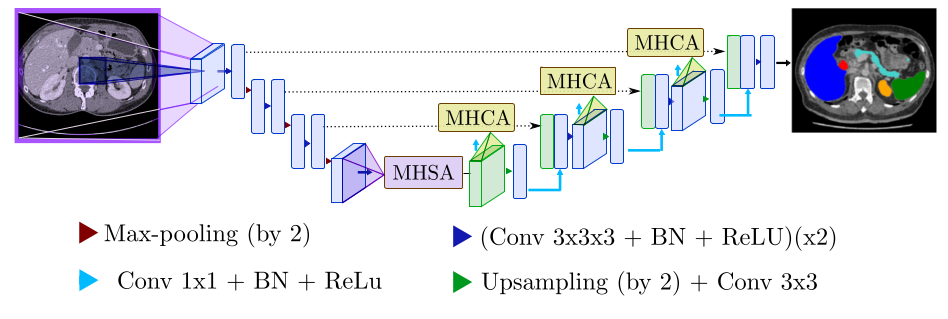
\includegraphics[scale=0.5]{ann19_arch.png} \\
        \captionof{figure}{\scriptsize{
            Архитектура U-Transformer.
        }}
    \end{center}
    
\end{minipage} 
\subsection*{Данные}
TCIA - публичный датасет снимков поджелудочной железы.\\
Датасет снимков внутренних органов (IMO).
\subsection*{Результаты}


{\small 
\begin{center}
    \captionof{table}{
            Результаты по метрике Dice.}

    \begin{tabular}{l|cc|ccc}
        \toprule[1pt]
        Dataset & U-Net & Attn U-Net & MHSA & MHCA & U-Transformer \\
        \hline
        TCIA & 76.13 ($\pm$ 0.94) & 76,82 ($\pm$ 1.26) & 77.71 ($\pm$ 1.31) & 77.84 ($\pm$ 2.59) & \textbf{78.50} ($\pm$ 1.92) \\
        IMO & 86.78 ($\pm$ 1.72) & 86.45 ($\pm$ 1.69) & 87.29 ($\pm$ 1.34) & 87.38 ($\pm$ 1.53) & \textbf{88.08} ($\pm$ 1.37) \\
        \toprule[1pt]
    \end{tabular}



\end{center}
}


{\small 
\begin{center}
    \captionof{table}{Результаты по каждому органу по метрике Dice на датасете IMO.}
    \begin{tabular}{l|cc|ccc}
        \toprule[1pt]
        Organ & U-Net& Attn U-Net & MHSA & MHCA & U-Transformer \\
        \hline
        Pancreas & 69.71 \footnotesize{($\pm$ 3.74)} & 68.65 \footnotesize{($\pm$ 2.95)} & 71.64 \footnotesize{($\pm$ 3.01)} & 71.87 \footnotesize{($\pm$ 2.97)} & \textbf{73.10} \footnotesize{($\pm$ 2.91)} \\
        Gallbladder & 76.98 \footnotesize{($\pm$ 6.60)} & 76.14 \footnotesize{($\pm$ 6.98)} & 76.48 \footnotesize{($\pm$ 6.12)} & 77.36 \footnotesize{($\pm$ 6.22)} & \textbf{78.32} \footnotesize{($\pm$ 6.12)} \\
        Stomach & 83.51 \footnotesize{($\pm$ 4.49)} & 82.73 \footnotesize{($\pm$ 4.62)} & 84.83 \footnotesize{($\pm$ 3.79)} & 84.42 \footnotesize{($\pm$ 4.35)} & \textbf{85.73} \footnotesize{($\pm$ 3.99)} \\
        Kidney(R) & 92.36 \footnotesize{($\pm$ 0.45)} & 92.88 \footnotesize{($\pm$ 1.79)} & 92.91 \footnotesize{($\pm$ 1.84)} & 92.98 \footnotesize{($\pm$ 1.70)} & \textbf{93.32} \footnotesize{($\pm$ 1.74)} \\
        Kidney(L) & 93.06 \footnotesize{($\pm$ 1.68)} & 92.89 \footnotesize{($\pm$ 0.64)} & 92.95 \footnotesize{($\pm$ 1.30)} & 92.82 \footnotesize{($\pm$ 1.06)} & \textbf{93.31} \footnotesize{($\pm$ 1.08)} \\
        Spleen & 95.43 \footnotesize{($\pm$ 1.76)} & 95.46 \footnotesize{($\pm$ 1.95)} & 95.43 \footnotesize{($\pm$ 2.16)} & 95.41 \footnotesize{($\pm$ 2.21)} & \textbf{95.74} \footnotesize{($\pm$ 2.07)} \\
        Liver & 96.40 \footnotesize{($\pm$ 0.72)} & 96.41 \footnotesize{($\pm$ 0.52)} & 96.82 \footnotesize{($\pm$ 0.34)} & 96.79 \footnotesize{($\pm$ 0.29)} & \textbf{97.03} \footnotesize{($\pm$ 0.31)} \\
        \toprule[1pt]
    \end{tabular}
\end{center}


}

\subsubsection*{Заключение}
В данной работе была предложена сеть U-Transformer, которая расширяет U-Net подобную 
полносвязную сеть трансформером. Рассмотренный метод показывает лучщие результаты 
по сравнению с уже существующими решениями. В дальнейшем авторы планирую изучать 
U-Transformer'ы в трехмерном случае на снимках различной модальности.